%=============================================================
\section{Introduction}
\label{sec:intro}
%=============================================================

Electroencephalogram (EEG) foundation models (FMs) have recently achieved strong transfer across clinical tasks including seizure detection, sleep staging, pathology classification, and emotion recognition~\citep{labram,eegpt,cbramod,biot,reve}. Scaling the pretraining corpus beyond the ${\sim}25{,}000$ hours available to the strongest open models is blocked not by compute but by \emph{data}: hospitals hold vast unlabeled EEG recordings but are reluctant to share them because the raw signals carry biometric fingerprints that enable subject re-identification~\citep{eeg_biometric_survey,fallahi2026eeg_biometric,eeg_reidentification}.

Learned privacy filters that apply a bounded perturbation to the signal have emerged as the natural interface for data release~\citep{unlearnable_eeg_meng,adversarial_filter,wang2025idremovalnet}. A filter takes raw EEG $X$ and returns $\Xt = X + \delta\cdot\tanh(G_\theta(X))$ with an architecturally enforced $\ell_\infty$ bound, trained adversarially against a subject-identification attacker while preserving a surrogate utility signal such as masked autoencoder (MAE) reconstruction~\citep{mae}. However, two structural problems remain open.

\textbf{Problem A: cross-dataset transfer is weak.} A filter trained on one source corpus frequently fails to generalize. In prior measurements on the NeuroVeil~v4 baseline, zero-shot cross-dataset adjusted privacy gain (APG) drops from $83.7\%$ on TUAB to $15.4\%$ on TUSL and $42.9\%$ on HMC~\citep{neuroveil_v4}. The TUSL failure is particularly diagnostic: TUSL shares TUAB's 19-channel montage but was not in the filter's training distribution, pointing to a filter reliance on source-site-specific artifacts.

\textbf{Problem B: the utility surrogate is paradigm-specific.} Half of modern EEG FMs use a vector-quantized (VQ) tokenizer as the pretraining target---LaBraM~\citep{labram} with an 8192-code neural tokenizer, CodeBrain~\citep{codebrain} with dual temporal+frequency codebooks, TFM-Tokenizer~\citep{tfm_tokenizer}, NeuroLM. A filter whose utility loss is raw MSE provides no signal about nearest-neighbor codebook assignments; StableToken~\citep{stabletoken} showed in speech that bounded-$\ell_\infty$ perturbations can flip VQ code indices arbitrarily even at tight MSE. The two structural problems are orthogonal but must be solved in the same artifact if the filter is to serve as the interface to the entire EEG-FM ecosystem rather than any single teacher.

\begin{figure}[t]
\centering
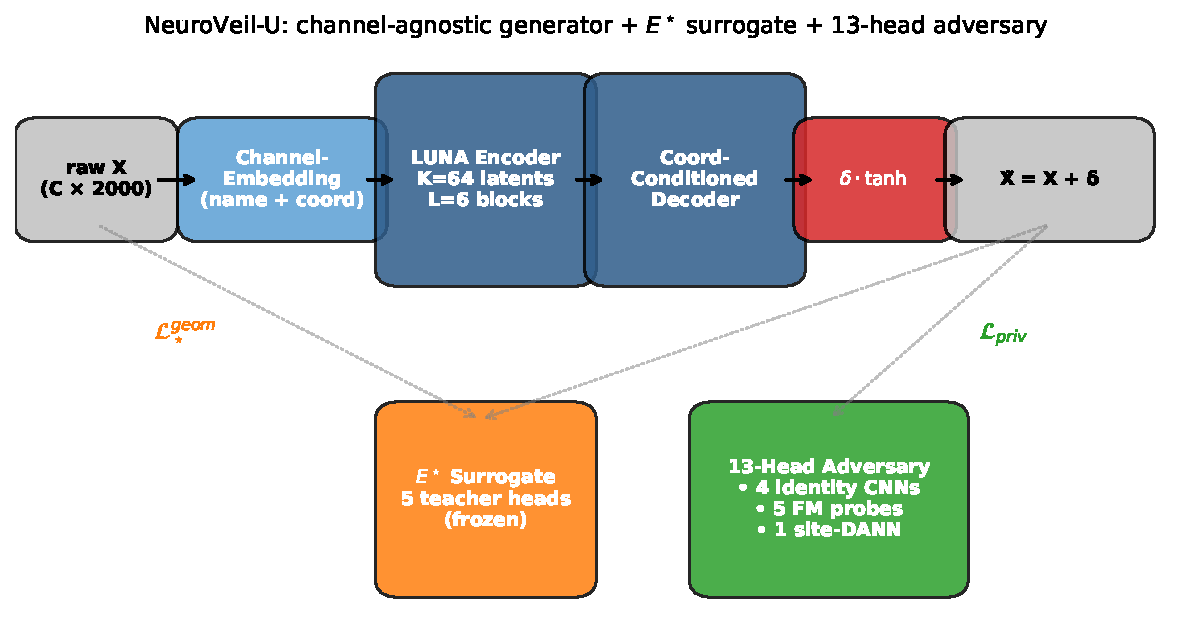
\includegraphics[width=\linewidth]{figures/fig_architecture.pdf}
\caption{\textbf{NeuroVeil-U architecture.} A \emph{channel-agnostic LUNA generator} with $K{=}64$ learned latent queries ingests any subset of the standard 10--05 channels embedded jointly with MNE Cartesian coordinates. An \emph{Ensemble Functional Surrogate} $\Estar$ distilled offline from five heterogeneous EEG foundation models covering three pretraining paradigms (continuous MAE, VQ tokenization, contrastive) carries the utility-preservation objective into a single student-forward pass. A 13-head adversary suite (four identity CNNs, five FM-representation probes, one site-DANN over 64 TUEG pseudo-sites) drives the privacy objective.}
\label{fig:arch}
\end{figure}

We propose \textbf{NeuroVeil-U}, a single bounded-perturbation filter whose thesis is that EEG privacy filtering should operate in the \emph{shared functional space} that all EEG-FM pretraining objectives consume. Three architectural moves combine into one training run.

\emph{(i) Channel-agnostic generation.} The filter's backbone is a LUNA-style~\citep{luna} encoder--decoder with $K{=}64$ learned latent queries. Each channel is embedded as the sum of a learned name-vocabulary token and an MLP of its MNE standard-1005 3-D coordinate. Training-time montage subsampling $C_{\text{sub}}\!\sim\!\mathrm{Uniform}(8,19)$ lets the single generator transfer zero-shot to any subset of standard-10--05 electrodes, including HMC's 4-channel bipolar montage.

\emph{(ii) Ensemble Functional Surrogate.} We distill one multi-head student $\Estar$ from a five-FM ensemble $\FMset\!=\!\{\text{BIOT}, \text{LaBraM}, \text{CBraMod}, \text{CodeBrain}, \text{REVE}\}$ covering three pretraining paradigms. Each teacher contributes an objective-matched head: L2-regression for continuous-MAE teachers; soft-KL over top-$K$ nearest codes for VQ teachers; and cosine projection for BIOT's contrastive head. Preserving $\Estar$'s geometry between $X$ and $\Xt$ then serves as a differentiable proxy for preservation in all teachers simultaneously, amortizing what would otherwise require five expensive FM forward passes per training step.

\emph{(iii) Thirteen-head adversarial suite with site-DANN and FM probes.} Beyond the four signal-space identity CNNs standard in prior work, we add one MLP probe on each frozen $E_F(\Xt)$ targeting subject identity and a gradient-reversal head predicting TUEG pseudo-site (hospital~$\times$~year $\to$ 64 classes). The filter's privacy loss is a soft-min worst-case across the identity attackers, and the site-adversarial objective explicitly discourages source-site-specific perturbations.

\textbf{Empirical results.} At a 1{,}000-subject TUEG training scale on a single A40 GPU ($\sim\!95$ minutes of Phase-2 training), the full NeuroVeil-U pipeline simultaneously: (a) reduces same-dataset re-identification on TUEG val from $78.72\%$ to $25.94\%$ (\textbf{APG $67.10\%$}, 338 subjects, retrained DeepCNN, perturbation RMS $1.55$, mean channel correlation $0.60$); (b) delivers \textbf{$80.41\%$ average cross-dataset APG} zero-shot on TUSL (APG $72.48\%$, 19ch matched) and HMC (APG $88.33\%$, 4-channel bipolar montage unseen during training)---a level the channel-agnostic generator and site-DANN head specifically target; and (c) preserves linear-probe utility on all five foundation-model teachers on TUAB within $6\%$ of the unfiltered baseline simultaneously (average utility ratio $0.955$: BIOT $0.954$, LaBraM $0.968$, CBraMod $0.964$, CodeBrain $0.946$, REVE $0.941$). An ablation (Section~\ref{sec:ablation}) isolates the training-schedule contribution: moving from a light configuration to our V4-aligned recipe lifts TUEG APG $1.1\%\!\to\!67.1\%$ and cross-dataset APG $3.4\%\!\to\!80.4\%$ with a $4.4$ percentage-point FM-utility cost. Our contributions are: a formulation of EEG privacy filtering as preservation of the shared latent geometry of a heterogeneous FM ensemble, an offline-distilled surrogate $\Estar$ that makes this preservation tractable in a single forward pass, a channel-agnostic LUNA-style generator with MNE standard-1005 coordinate embedding, a site-adversarial head over 64 TUEG pseudo-sites, and an open-source 13-head attacker-retrained evaluation protocol that extends the standard 4-attacker ensemble with FM-representation probes.
